\documentclass{standalone}
\usepackage{tikz}
\usepackage{tikz-qtree,tikz-qtree-compat}

\begin{document}

\tiny
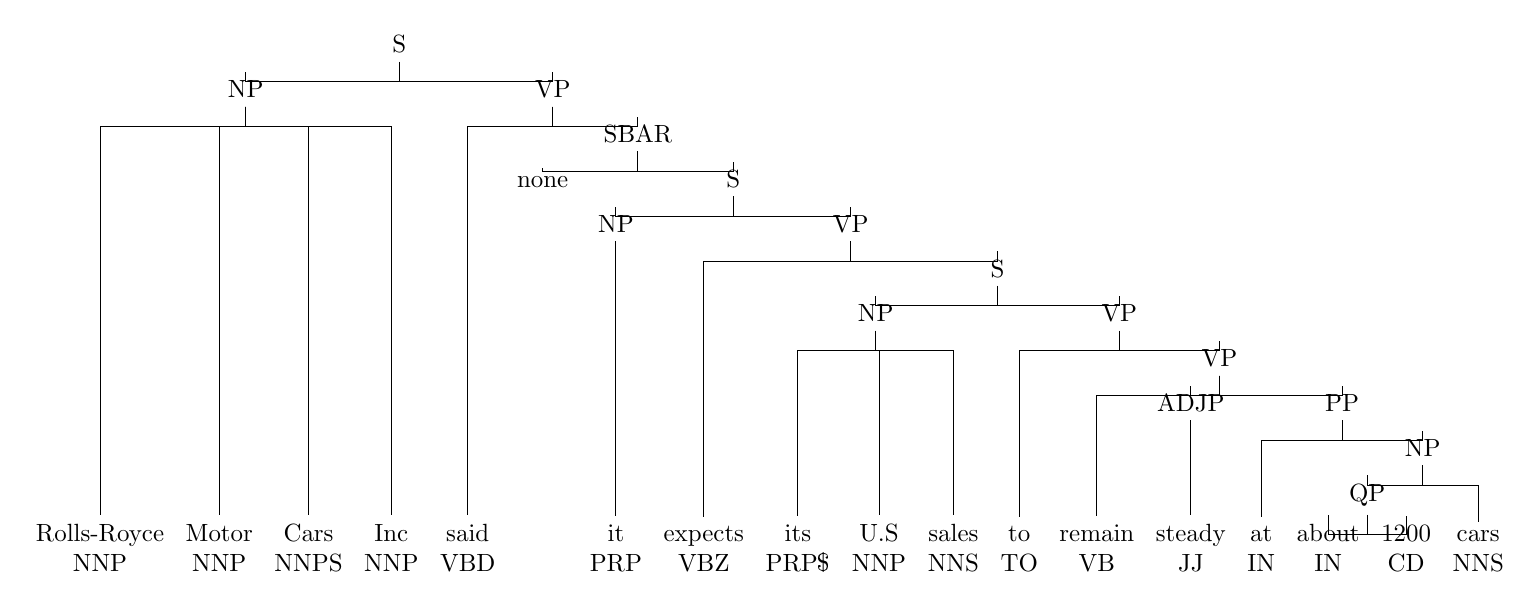
\begin{tikzpicture}[every node/.style={align=center},scale=.9]
  \tikzset{
    edge from parent/.style={
      draw,edge from parent
      path={(\tikzparentnode.south)-- +(0,-8pt)-| (\tikzchildnode)}
    },
    frontier/.style={distance from root=208pt}, % Align leaf nodes
    level 1+/.style={level distance=18pt} % Distance between levels
  }

   \Tree [.S
             [.NP Rolls-Royce\\NNP Motor\\NNP Cars\\NNPS Inc\\NNP ]
             [.VP said\\VBD
                [.SBAR [.none ]
                   [.S
                      [.NP it\\PRP ]
                      [. VP expects\\VBZ
                         [.S
                            [.NP its\\PRP\$ U.S\\NNP sales\\NNS ]
                            [.VP to\\TO
                               [.VP remain\\VB
                                  [.ADJP steady\\JJ ]
                                  [.PP at\\IN
                                     [.NP
                                        [.QP about\\IN 1200\\CD ]
                                        cars\\NNS
                                     ]
                                  ]
                               ]
                            ]
                         ]
                      ]
                   ]
                ]
             ]
         ]
\end{tikzpicture}
\end{document}